\paragraph{Evidence design.}
Oracle Gaussian and mixture factors isolate subsampling from score learning. Five mixture density networks then test compositions of learned conditional densities with known Gaussian tails. Each network completes 40,000 training updates; reference posterior labels are not used for training. A third family has nonorthogonal observations and analytically available nonseparable posterior mixtures. Sampling time includes method-specific preparation, transfer and resampling. One-time prediction of learned factor parameters and construction of common reference distributions are reported separately. The networks are evaluated once per dataset; subsequent factor scores are analytic mixture calculations.

\subsection{Finite samples can conceal a divergent population update}
In the four-factor example of \eqref{eq:counterexample}, every finite with-replacement batch size has an infinite normalizer. With $1{,}048{,}576$ particles, increasing $M$ from 2 to 32 nevertheless lowers mean potential MSE from $0.46798$ to $0.01857$ and increases median ESS fraction from $0.000424$ to $0.932706$. At $M=32$, all 20 runs miss the nonintegrable batch events. The observed mean log normalizer is $0.126047$ with standard deviation $0.000259$, close to the exact full-factor value $0.122049$. The theorem supplies the divergence statement; finite observations illustrate its limited visibility.

\begin{figure}[t]
\centering
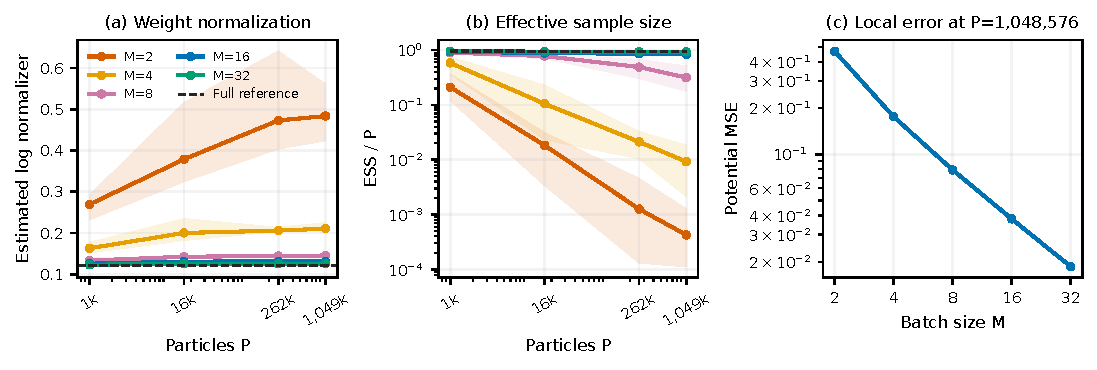
\includegraphics[width=\linewidth]{figures/one_step.pdf}
\caption{The exact divergence certificate is unchanged as batch size grows. Finite-particle normalizer estimates and ESS can nevertheless appear stable. Panels show medians and interquartile ranges over 20 runs, with mean potential MSE and one standard deviation at the largest particle count.}
\label{fig:paper-one-step}
\end{figure}

The full-factor Euler scheme also has a finite-step boundary. At $G=64,K=128$, the ordinary Gaussian benchmark has a negative denominator, while observed eight-dimensional W1 is only $0.0176$. Conversely, finite configurations can have substantial particle error. For a separate 16-step Gaussian path, the exact first weight moment is finite and the second infinite (Appendix~\ref{app:dual-results}). Existence, second moments and observed error are separate diagnostics.

\subsection{Tail control and useful posterior accuracy}
The fixed benchmark includes 1,980 oracle cells, followed by 1,080 oracle-extension and 1,000 learned sampling cells. In the learned study, all 600 full or tail-controlled cells have finite normalizers; all 400 raw subsampled cells are divergent. The largest setting uses $G=64,d=8,N=32768,K=2048$. W1 against the learned composition is $0.0189$ for full weighting and $0.0907$ for fixed-mean tail control without replacement. Thus restoring the finite domain alone does not solve the accuracy problem.

Anchoring reduces this fixed-mean control error on a separately held-out cohort: W1 changes from $0.09539$ to $0.01967$, compared with full weighting at $0.01682$. An equivalent implementation takes $3.844$ seconds against $6.039$ for full weighting. Its W1 degradation upper bound is $0.00608$, exceeding the declared $0.002$ allowance. On the same saved particles, observed 90\% interval coverage improves from $66.00\%$ to $87.25\%$, with full weighting at $88.50\%$. These ten data seeds and five trained models do not establish general calibration. Appendix~\ref{app:dual-results} retains the complete-kernel correction ablations and all failed joint accuracy--cost criteria.

Product structure also matters. Coordinatewise full-factor SMC lowers W1 from $0.6973$ to $0.2703$ on the difficult product mixture; joint sign TV remains $0.3685$. This is a strong problem-specific baseline, with residual mode error. A fresh study uses eight development targets to select an anchored batch/particle/grid configuration and fixes it before evaluating five checkpoints crossed with twenty new datasets. The two-way paired bootstrap samples checkpoints and datasets separately. Results are assessed against both joint and coordinatewise full-factor baselines.

The selected configuration has $N=8192,K=1024,M=8$. On the 100 new model--dataset pairs, its W1 is $0.01908$ in $1.240$ seconds, compared with $0.01972$ in $6.097$ seconds for the original $N=32768,K=2048$ joint baseline. Its one-sided 95\% W1-degradation bound is $0.001323$, below the fixed $0.002$ allowance. Coordinatewise full weighting at the original budget achieves $0.01556$; the corresponding degradation bound is $0.005200$, so the predeclared requirement to pass both baselines fails.

A post-hoc same-cohort ablation gives both baselines the selected $N,K$ and replays the anchor. Full weighting then takes $1.404$ seconds at W1 $0.02076$, coordinatewise weighting $1.498$ seconds at $0.01667$, and the anchor $1.235$ seconds at $0.01908$. Thus the anchor's time reduction against joint weighting is about $12\%$ at equal particle/grid budgets; most of the apparent $4.9\times$ difference above is budget selection. Its W1-degradation upper bound against the matched coordinatewise baseline is $0.004199$, again exceeding $0.002$. This ablation reuses the same targets and supplies no additional independent data. Appendix~\ref{app:paper-level-results} gives the audit and intervals.

\subsection{A nonseparable inverse problem and a direct-likelihood baseline}
We observe $y_g=s_ga_g^\top\theta+\epsilon_g$ for twelve nonorthogonal unit directions, with $\theta\sim\Normal(0,I_d)$, uncertain sensor polarity $s_g\in\{-1,1\}$ and Gaussian noise. Each single-observation posterior is a two-component Gaussian mixture with shared covariance. Different directions produce noncommuting factor precisions and a nonseparable joint posterior. Enumeration of $2^{12}=4096$ sign patterns gives an exact mixture reference. This is a controlled sensing problem, not measured-sensor data or a demonstration of large-scale application benefit.

Eight development problems fix the control configuration and an annealed SMC baseline \citep{delmoral2006,cotter2013}. The latter uses the available likelihood, pCN moves and a Metropolis sign flip. Confirmation uses $d\in\{2,8\}$, two noise regimes and twenty new shared data seeds: eighty problems, with uncertainty resampled over the twenty seed clusters. Table~\ref{tab:sensor-main} reports mean W1 averaged over 32 fixed projections. Every full and tail-controlled cell has a strict matrix certificate, yet anchored control is inaccurate in the sharper regime; for $d=2$, its error is $0.8232$ against $0.02917$ for full weighting. Annealed SMC has the smallest non-oracle error. The reference-to-reference Monte Carlo discrepancy is $0.00420$. We exclude this study's wall-clock comparisons because another GPU task overlapped its final interval.

\begin{table}[t]
\centering\small
\caption{Nonseparable confirmation: eighty problems from twenty shared seeds. Brackets give seed-cluster bootstrap 95\% intervals. Coverage is observed marginal 95\% interval coverage, not a population calibration guarantee.}
\label{tab:sensor-main}
\begin{tabular}{lrr}
\toprule
Method & Projected W1 [95\% interval] & Coverage\\
\midrule
Full weighting & $0.02011\ [0.01594,0.02552]$ & $0.941$\\
Raw batch, $M=4$ & $0.02827\ [0.01914,0.04055]$ & $0.933$\\
Fixed-mean tail control & $0.39501\ [0.28349,0.50539]$ & $0.848$\\
Anchored tail, $M=8$ & $0.23623\ [0.13908,0.34555]$ & $0.900$\\
Annealed SMC & $0.00715\ [0.00669,0.00780]$ & $0.945$\\
Exact-mixture draws & $0.00650\ [0.00614,0.00692]$ & $0.945$\\
\bottomrule
\end{tabular}
\end{table}

Finally, a separate eight-problem development pilot evaluates the tail-matched Gaussian path proposal with exact transition-density correction. Although Theorem~\ref{thm:gaussian-twist-moments} guarantees all fixed positive weight moments, the best mean-error Gaussian-mixture proposal has projected W1 $0.12567$, compared with $0.02500$ for full weighting and $0.00702$ for annealed SMC. No candidate meets the fixed joint accuracy--cost gate, so the protocol stops expansion. This result distinguishes existence of high moments from useful mode coverage and finite-sample efficiency.
